\documentclass[a4paper,10pt]{article}
\usepackage[utf8]{inputenc}
\usepackage[T1]{fontenc}
\usepackage[french]{babel}
\usepackage{graphicx}
\usepackage[font=small,labelfont=bf]{caption}
\usepackage{amsmath}
\usepackage{stackengine}
\usepackage{setspace}
%\usepackage{placeins}

\newcommand\tabA[1][0.5cm]{\hspace*{#1}}
\newcommand\tabB[1][1.5cm]{\hspace*{#1}}
\newcommand\tabC[1][2cm]{\hspace*{#1}}
\setlength{\parindent}{0cm}
\setlength{\parskip}{1ex plus 0.5ex minus 0.2ex}
\newcommand{\hsp}{\hspace{20pt}}
\newcommand{\HRule}{\rule{\linewidth}{0.5mm}}


% Title Page
\begin{document}
\begin{titlepage}
  \begin{sffamily}
  \begin{center}

    % Upper part of the page. The '~' is needed because \\
    % only works if a paragraph has started.
    
\includegraphics{./image/ua_v_couleur.jpg}
    
    \textsc{ UNIVERSIT\'{E} D'ANGERS \\ UFR INFORMATIQUE}\\[0.5cm]
    \textsc{ \\ Rapport de stage \\ Master 1 2016-2017 }\\[1.5cm]
    
    
\includegraphics{./image/logo-generique-SD.png}
    
    \textsc{UMR INSERM 1232 \\-Equipe Immunité Innée et Immunothérapie}\\[1cm]
     
    % Title
    \HRule \\[0.4cm]
    { \huge \bfseries ANALYSE TRANSCRIPTOMIQUE\\[0.4cm] }

    \HRule \\[2cm]
    \centering\vspace*{\fill}
    \begin{minipage}{9\textwidth}
    \begin{doublespace}
    \begin{tabular}{cl}
       \large Présenté par : &\tabC \tabA \textsc{RASOLONIAINA Marlino}\\
       \newline
       \emph{Maître de stage  :} &\tabC \tabA Dr. \textsc{Valérie Seegers}\\
       \emph{Responsable d'équipe : } &\tabC \tabA Dr.  \textsc{Yves Delneste} \\
       
    \end{tabular}
     \end{doublespace}
    \emph{Laboratoire d'accueil :} \tabC \tabA \textsc{INSERM U1232}-Equipe 7
    \\\tabC \tabC \tabC \tabA Bâtiment IRIS 
    \\\tabC \tabC \tabC \tabA CHU-4,rue Larrey 
    \\\tabC \tabC \tabC \tabA 49933 ANGERS
    \end{minipage}
    \vspace*{\fill}
     % Author and supervisor
%      \begin{minipage}{0.4\textwidth}
%        \begin{flushleft} \large
%          \large Présenté par : \\\textsc{RASOLONIAINA Marlino}
%        \end{flushleft}
%      \end{minipage}
%      \begin{minipage}{0.4\textwidth}
%        \begin{flushright} \large
%          \emph{Maître de stage  :} Dr. \textsc{Valérie Segers}\\
%          \emph{Responsable d'équipe : } Dr.  \textsc{Yves Delneste}
%        \end{flushright}
%      \end{minipage}
%  
%      \vfill

    % Bottom of the page
    {\large 12 Avril 2017 — 20 Juin 2017}

  \end{center}
  \end{sffamily}
\end{titlepage}
\newpage
\tableofcontents
\newpage
\section{INTRODUCTION :}
Besoin d'inspiration
\section{PR\'{E}SENTATION DE L'ORGANISME D'ACCUEIL :}
\subsection{Présentation générale (activité, organisation, services...) :}
\subsection{Présentation du service rattaché :}
\section{PR\'{E}SENTATION DU SUJET DE STAGE :}
\subsection{Objet et missions du stage :}
\subsection{Missions réellement réalisées :}
\section{ACQUISITION DES DONN\'{E}ES :}

\subsection{ Plan expérimental :}
Le sujet du stage s’inscrit dans la thématique principale du laboratoire qui porte sur l’adaptation du macrophage aux modifications environnementales et plus précisément : l’impact de la présence d’acide lactique (AL), qui s’accumule au sein des tumeurs, sur l’expression génique des macrophages de type M1 (pro-inflammatoires et initiateurs de la réponse immunitaire) et de type M2 (immunotolérants et qui s’accumulent dans les tissus cancéreux).

Pour répondre à cette question, le laboratoire modélise in vitro la polarisation des macrophages en modifiant les conditions de culture des cellules envisageant ainsi 8 conditions expérimentales. (Graphique) Comme il y avait 3 donneurs différents, 24 prélèvements ont été préparés et analysés sur les puces ADN.

Les questions biologiques à explorer sont les suivantes : Quels gènes sont différentiellement exprimés par les macrophages  G (M1) et par les macrophages M (M2) en présence d’acide lactique (AL), en dehors de toute stimulation par LPS ? Avec une stimulation par LPS ? Quels sont les processus biologiques concernés par l’exposition des macrophages à l’acide lactique ? Quelles sont les voies de signalisation concernées ?
\begin{center}
 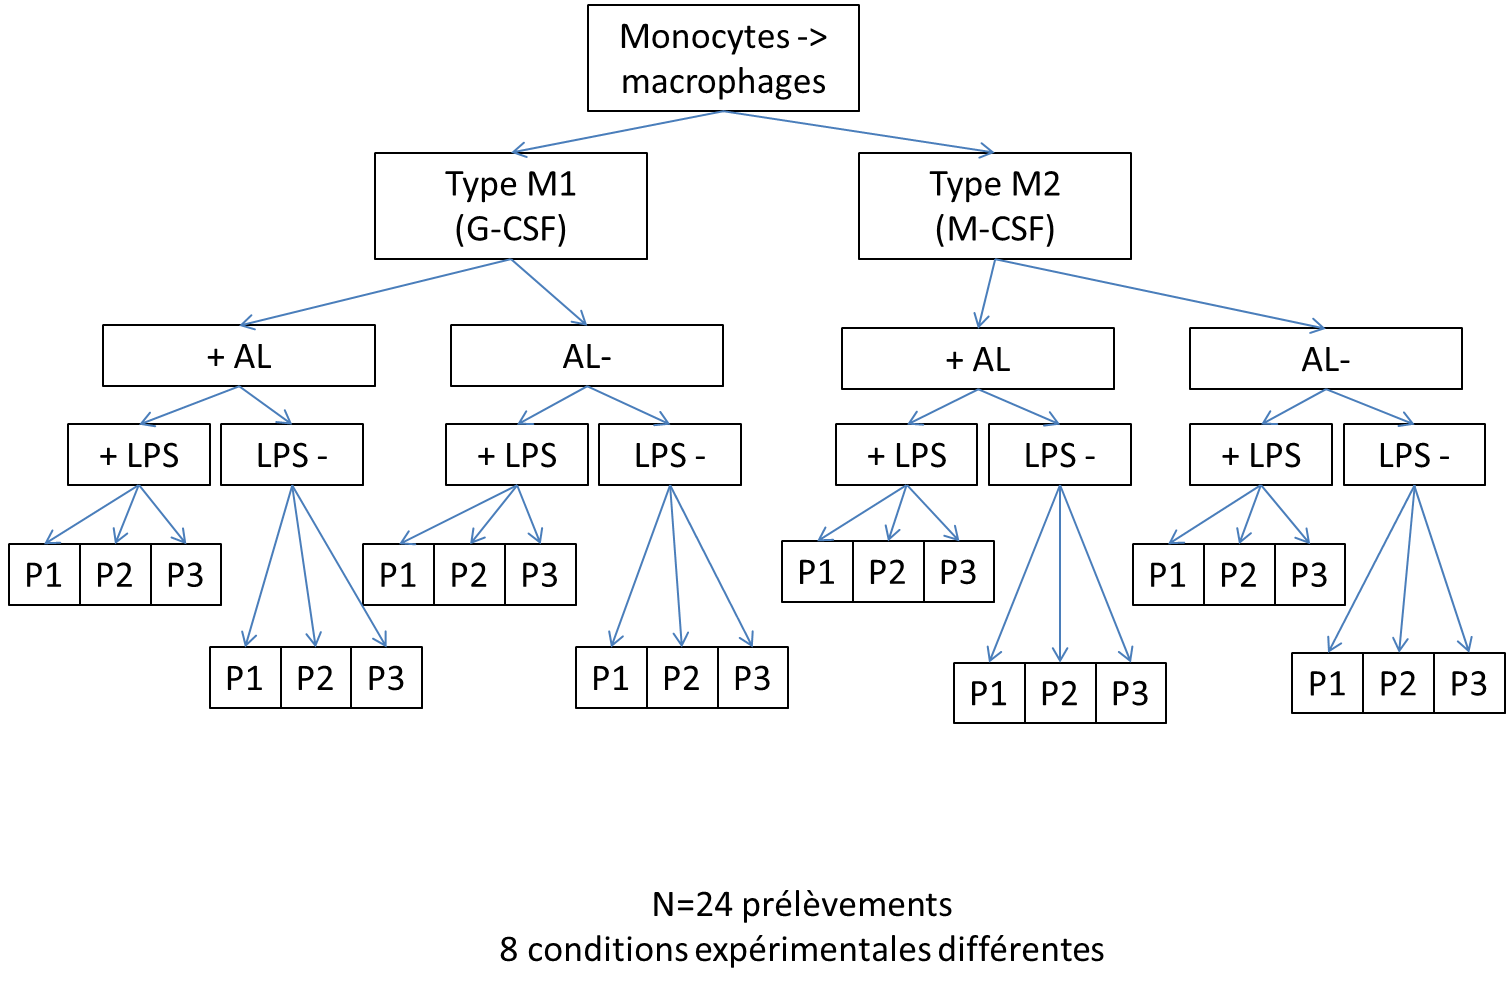
\includegraphics[scale=0.5]{./image/plan.png}
 % plan.png: 0x0 pixel, 300dpi, 0.00x0.00 cm, bb=
 \captionof{figure}{Plan éxpérimental }
\end{center}
L’expérience a été faite avec la puce ADN  Illumina HumanHT-12 v4.0 BeadChip 12x1 avec 48210 sondes pour chaque prélèvement.
887 de ses sondes sont classés comme des sondes de contrôles.
On se trouve donc avec 47323 individus sur 24 variables. 
Ce qui nous donne une matrice de données de dimension :
\def\tmp{
  \begin{pmatrix}
  a_{11} & \cdots & a_{1m} \\

   \vdots & \ddots &\vdots \\

   a_{n1} & \cdots & a_{nm} 
 \end{pmatrix}
}
\[
\stackMath\def\stackalignment{r}
  \stackon
    {\mathrm{47323~rows}\left\{\tmp\right.}
    {\overbrace{\phantom{\smash{\tmp\mkern -36mu}}}^{\mathrm{\textstyle 24~columns}}\mkern 20mu}
\]

\subsection{Les puces à ADN :}
  Une puce à ADN est constituée d'un support physique (le plus
  souvent une lame de verre) sur lequel sont déposées des molécules
  d'ADN correspondant à de petits fragments du génome (jusqu'à 40 000
  dépôts différents par puce). On recouvre la puce
  de la solution contenant la population d'ARN à étudier. Les ARN
  s'hybrident sur les fragments d'ADN complémentaires. La quantité d'ARN
  fixée reflète la concentration de cet ARN dans la solution.
  \newline
 Pour des raisons pratiques, on utilise de l’ADN complémentaire plutôt que directement
  l'acide ribonucléique car l’ADN est plus stable. Les ADNc sont marqués par un nucléotide radioactif ou
  un fluorochrome. Il est possible d'étudier simultanément plusieurs
  populations d'ADNc sur une même puce en utilisant des fluorochromes différents.
  La meilleure façon d'utiliser cette possibilité est de marquer
  l'ADN génomique avec un fluorochrome, toujours le même. On
  obtient ainsi une référence stable au cours des années
  qui permet de mettre toutes les puces à la même échelle,
  quelle que soit leur origine. 
  \newline
  Un scanner mesure l'intensité du signal émis par l'ADNc hybridé au niveau de chaque dépôt. Parmi les valeurs que proposent les
  logiciels pour cette intensité, la plus fiable est la médiane de l'intensité des pixels car elle est moins sensible aux défauts de
  l'image (pixels sur-brillants par exemple). 
  \newline
  Les puces comportent généralement plusieurs dépôts identiques pour chaque gène. Cela simplifie le travail lorsqu'il faut
  repérer les aberrations dans la lecture des intensités puisqu'il suffit d'examiner les cas où les valeurs diffèrent beaucoup d'un
  dépôt à l'autre. Il s'agit le plus souvent d'un défaut physique sur la puce et il est facile d'éliminer la valeur aberrante.
  Dans le doute, on conserve la médiane des différentes mesures. 
  \newline
  Plusieurs  types  de  puces  à  ADN  
existent selon le support, la nature des fragments fixés à la surface, le mode de fabrication, la 
densité, le mode de marquage des cibles et les méthodes d’hybridation.
On sait que toutes les technologies des puces ADN se basent sur le principe fondamental de l’hybridation complémentaire des brins d’acide nucléique même si leurs techniques se diffèrent largement entre-elles, 
par exemple sur la longueur et la type de la sonde utilisée (cDNA arrays, oligonucleotide array), l’étiquetage et le protocole d’hybridation…
La vraie différence entre ces approches résident sur la précision, la spécificité, la sensibilité et la robustesse de chaque plateforme.
\begin{center}
 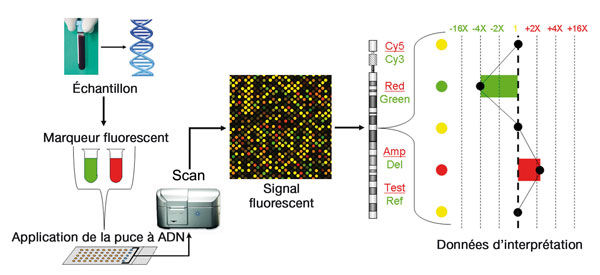
\includegraphics[scale=0.5]{./image/principe.jpg}
 % Etapes_d'une_expérience_de_biopuces.png: 0x0 pixel, 300dpi, 0.00x0.00 cm, bb=
 \captionof{figure}{Principe général d'utilisation des puces ADN }
\end{center}

\subsection{La technologie Illumina :}
Illumina, Inc. est une société américaine qui fabrique et commercialise des systèmes intégrés pour l'analyse de la variation génétique et la fonction biologique, 
notamment des gammes de produits et services qui servent les marchés du séquençage, génotypage et expression génétique.
\newline
Une de ces récentes fabrications est la puce ``BeadArray technologie''.
\begin{center}
 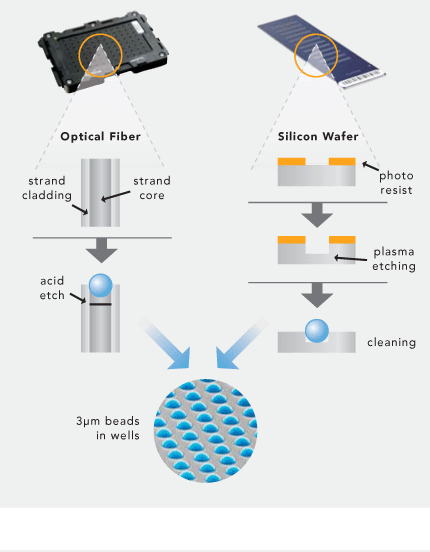
\includegraphics[scale=0.5]{./image/beadarray.png}
 % beadarray_multi_sample_array_formats_lg.gif: 0x0 pixel, 300dpi, 0.00x0.00 cm, bb=
 \captionof{figure}{Illumina BeadArray Technologie }
\end{center}
Dans l’analyse des expressions des gènes, Illumina utilise deux approches différentes : l’hybridation directe(Direct Hybridization assay) et le DASL (cDNA-mediated Annealing Selection Extension and Ligation).
L’expérience est faite avec la première approche qui consiste à utiliser un simple brin de la séquence d’ADN (pour chaque sonde). Cette séquence monocaténaire s’hybride avec la séquence cible étiquetée dans l’échantillon. 
La quantité du signal fluorescent produit détermine la quantité de l’ARN cible dans l’échantillon.
\begin{center}
 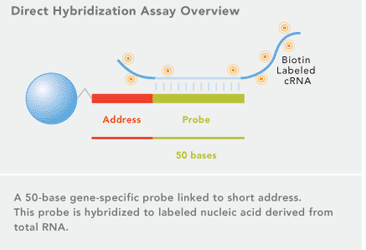
\includegraphics[scale=0.5]{./image/Direct_Hyb.png}
 % direct_hybridization_assay_workflow_lg.png: 0x0 pixel, 300dpi, 0.00x0.00 cm, bb=
 \captionof{figure}{An Illumina Direct Hybridization probe }
\end{center}
\begin{center}
 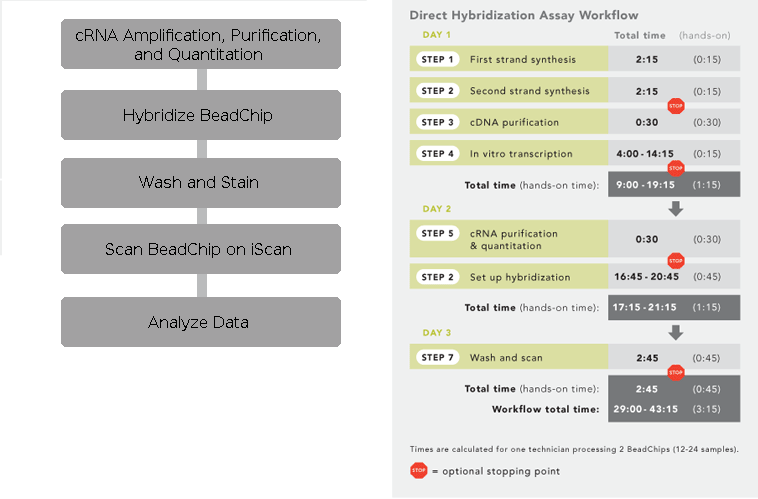
\includegraphics[scale=0.5]{./image/direct_hybridization_assay_workflow.png}
 % direct_hybridization_assay_workflow.png: 0x0 pixel, 300dpi, 0.00x0.00 cm, bb=
 \captionof{figure}{ Direct Hybridization assay workflow}
\end{center}

\subsection{Les sources de variations et les défis sur l'utilisation des puces ADN :}

En Biologie,si on effectue à plusieurs reprises une même expérience, on peut se heurter à des valeurs d’expérience légèrement différentes à chaque exécution.
Il est de ce fait très intéressant de voir de plus près les grandes étapes et les effets des processus biologiques qui sont derrières ces sources de quantité de variabilité dans l’étude des expressions génomique avec les puces ADN.
De ce point de vue, ces variations sont considérées comme des bruits dans la phase d’analyse des expressions.\\
Est-ce que la variation d’un gène particulier est due au bruit de fond de la puce ou c’est réellement une différence entre les conditions expérimentales? C’est là le vrai defi. 
Si on prend un gène spécifique, combien de quantité de sa valeur représente la mesure de la variance due à la régulation des gènes et due à la quantité de bruit ?
Ces sources de variation (Tableau :~\ref{Sources de variation}) nous mènent aux problèmes de fiabilité et de reproductibilité dans les mesures des puces ADN qui sont souvent négligés.
Néanmoins, une grande partie de la variabilité induite par la puce elle-même  peut être déterminée à l'aide des techniques 
de réplications ou d’autres techniques de séparations des bruits (Exemples : conception d’expérience statistique, normalisation des données).
Plusieurs efforts ont été menés pour évaluer la fiabilité, la précision et la reproductibilité des puces ADN, inclus des projets comme MAQC(MicroArray Quality Control). \\

\begin{table}[!ht]
\centering
\begin{tabular}{|p{3cm}|p{9cm}|}
\hline
 \emph{Facteur} & \emph{Commentaires}\\
\hline
Préparation des mRNA  &  Tissus, les kits et les procedures variantes \\
\hline 
Transcription & Les variations inhérentes dans la réaction, le type de l'enzymes utilisé  \\
\hline 
L'étiquetage (Labeling) & Depend du type,des procédures et l'âge de l'étiquette  \\
\hline
Amplification (PCR) & Il est difficille de quantifier le rendement du PCR\\
\hline
Variations géométriques des broches & différentes surfaces et propriétés dues à des erreurs aléatoires de production \\
\hline
Volume de l'échantillon & fluctue stochastiquement même pour la même broche (pin)  \\
\hline
Fixation de l'échantillon & La fraction de l'ADNc cible (une gouttelette) qui est chimiquement liée à la surface de la diapositive n'est pas prise en compte \\
\hline
 Paramètre d'hybridation &  influencé par plusieurs facteurs comme la temperature,le temps,le buffering \\
\hline
 Hybridation non-spécifique & un ADNc s'hybride avec une sequence qui n'est pas exactement son complémentaire \\
\hline
Réglages de gain & déplace la répartition des intensités de pixels \\
\hline
Limitation de la plage dynamique & Variabilité de la saturation au bas de gamme ou au haut de gamme \\
\hline
Alignement d'image & Les images d'un même BeadArray à diverses longueurs d'onde correspondant à des canaux différents ne sont pas alignées; différents pixels sont considérés pour le même emplacement \\
\hline
 Placement de la grille & le centre du spot n’est pas bien localisé  \\
\hline
 Bruit de fond non-spécifique& Élévation erronée de la moyenne de l'intensité du bruit de fond \\
\hline
Forme de spot & L'intensité des spots irréguliers sont difficille à segmenter en bruit de fond \\
\hline
 Segmentation & Des contaminants lumineux peuvent ressembler comme un signal(ex: poussière) \\
\hline
 Quantification de spot & la moyenne des pixels, la médiane,... \\
\hline
\end{tabular}
\caption{Sources of fluctuations in a typical cDNA microarray experiment}
\label{Sources de variation}
\end{table}
%\FloatBarrier
\section{DESCRIPTION DES DONN\'{E}ES :}
\subsection{ Décryptage et lecture :}
Après avoir scanné la puce, le scanner iScan d’Illumina exporte et produit des fichiers de sortie (Tableau :~\ref{Fichiers_Sorties}) .
Les fichiers qui contiennent les intensités de chaque sonde (.idat) sont encryptés et d’autres fichiers sont fournis à titre indicatif et de mesure pour l’analyse.\\
\begin{table}[!ht]
\begin{tabular}{|p{3cm}|p{9cm}|}
\hline
\emph{File}  & \emph{Description} \\
\hline
 (Serial Number).txt & un fichier qui stocke la positions et l'identité de chaque spots, qui contient quelques informations sur les paramètres du scanner\\
\hline
Metrics.txt &  un pour chaque BeadChip  et contient des informations récapitulatives sur l'intensité des signals,
la quantité de saturation, la mise au point et l'enregistrement sur l'image (s) de chaque section \\
\hline 
Effective.cfg & fichier de configuration des paramètres du scanner\\
\hline
(Serial Number).sdf & fichier de description des échantillons d'Illumina utilisé pour déterminer les propriétes (positions)
physique d'une section et savoir les sections liées sur chaque échantillons\\
\hline
*.idat & contiennent la moyenne des intensités du signal de chaque spots \\
\hline
\end{tabular}
\caption{Description des fichiers de sortie}
\label{Fichiers_Sorties}
\end{table}
\newline
Pour la lecture  des fichiers .idat, l’utilisation d’un fichier manifeste qui contient l’ensemble de tout les informations nécessaires concernant la puce est indispensable pour le décryptage : le nom et l’identifiant  des gènes ( Probe\_id, Array\_Address\_Id, Symbol, Barcode), le statut d’une sonde (regular, negative, biotin,...)
Dans la suite logique des choses, Illumina fourni un logiciel payant (GenomeStudio Software)  qui aide sur le traitement et l'analyse des puces ADN (Genotyping Module, Gene Expression Module, Methylation Module).
\subsection{ Données brutes via Bioconductor :}
Bioconductor est un projet de développement et un ensemble de package (1380 packages en 2017)  gratuit et open source dans l’analyse et la compréhension des données génomiques basé principalement en langage de programmation statistique R.
Limma est un des packages (de choix) dans Bioconductor pour l’analyse des expressions génomique des puces  ADN. La function read.idat de package Limma permet de lire les fichiers idat d’Illumina BeadArray en fournissant en paramètre le fichier manifeste .bgx correspondant à la plateforme d’expression de gène à étudier.
On obtient après un objet limma de type EListRaw  qui contient les objets suivants:
\begin{table}[!ht]
\begin{tabular}{|p{3cm}|p{9cm}|}
\hline
 \emph{E} & matrice des intensité brutes\\
\hline
\emph{other\$NumBeads }   &  matrice de mêmes dimensions que E donnant les nombre de spots (bead) utilisées pour chaque valeur d'intensité. \\
\hline 
\emph{other\$STDEV} & matrice de mêmes dimensions que E donnant un écart type au niveau des spots ou une erreur standard pour chaque valeur d'intensité.\\
\hline
\emph{genes} & un data.frame des annotations des sondes qui contient des informations extraites du fichier manifeste relatif au type de puce utilisé : Probe\_Id, Array\_Address\_Id, Status
\\
\hline
\end{tabular}
\caption{Contenu de l'objet EListRaw retourné par la fonction read.idat() de limma}
\label{EListRaw}
\end{table}
\subsection{ Contrôle et qualité :}
Par approximation, on peut considérer qu’un signal émis par la puce soit :
\begin{itemize}
 \item la vraie intensité produit par le gène cible
 \item un signal d’une hybridation non-spécifique
 \item un bruit de fond non-spécifique
\end{itemize}
La puce d’Illumina introduit alors des sondes appelées sonde de contrôle pour pouvoir mesurer et quantifier la qualité des données obtenues.
Avec ces sondes de contrôles, on peut quantifier les bruits et la qualité du signal, vérifier la qualité de la mesure d’expression de l'ensemble des sondes de la puce. 
Une valeur anormale produit par un seul BeadArray peut compromettre le résultat d’une analyse sur l’ensemble des données. 
On ne peut pas donc être assuré d’avoir un bon résultat en phase d’analyse si la qualité des données obtenues n’est pas acceptable (Tableau :~\ref{Control Dyrect  Hyb}).
\begin{table}[!ht]
\centering
\begin{tabular}{|p{3cm}|p{9cm}|}
\hline
 Contrôle de spécimen biologique & ces sont des gènes appelés ‘housekeeping genes’ qui doivent être exprimés dans tous les échantillons\\
\hline
Contrôle de l’étiquetage des échantillons (Labeling)   &  des ARN spécifiques(lysA,pheA,thrB,trpF) sont introduits dans les échantillons juste avant la transcription inverse (cDNA) et l’étiquetage. Des faibles signaux provenant de ses sondes indiquent des éventuelles problèmes lors de la réaction \\
\hline 
Contrôle de l’hybridation & 
\begin{itemize}
 \item Cy3-labeled hyb : ce contrôle se compose de 6 sondes d’oligonucléotides marqué par le fluorochrome Cy3 avec trois concentrations (low, medium, high) et doit produire des signaux progressivement croissants.
 \item Low-stringency hyb: ce contrôle de stringence d’hybridation se compose de 8 sondes (medium, high) avec exception que chaque sonde contient deux bases mésappariés  (Perfect Match \& Mismatch )
 \item High-stringency hyb
\end{itemize}
\\
\hline
Contrôle de génération des signaux & des ARN sont marqués par de la biotin. On attend un signal d'hybridation positif provenant de ces sondes\\
\hline
Contrôle de sonde négative & des centaines de sondes de séquences aléatoires sans cibles dans le génome sont intégrées dans la puce reflétant les signaux de bruit de fond du système d'imagerie,d'hybridation croisée et autres.On s'attend à des faibles signaux provenant de ces sondes. \\
\hline
\end{tabular}
\caption{Liste des contrôles des données d'Illumina BeadArray}
\label{Control Illumina}
\end{table}

\begin{table}[!ht]
\centering
\begin{tabular}{|p{3cm}|p{9cm}|}
\hline
 \emph{Métiques} & \emph{Valeurs attendues}\\
\hline
Hybridization Controls*   &  High > Medium > Low \\
\hline 
Low Stringency* & PM > MM2\\
\hline
Biotin and High Stringency* & valeurs élevées\\
\hline
Negative Controls (Background and Noise) & valeurs faibles \\
\hline
Gene Intensity (Housekeeping and All Genes) & Plus élevée que les bruits de fond (Housekeeping > All Genes) \\
\hline
Labeling and Background & Labeling >= Background \\
\hline
\end{tabular}
\caption{Contrôle d'hybridation direct de la technologie BeadArray d'Illumina}
\label{Control Dyrect  Hyb}
\end{table}
\begin{center}
 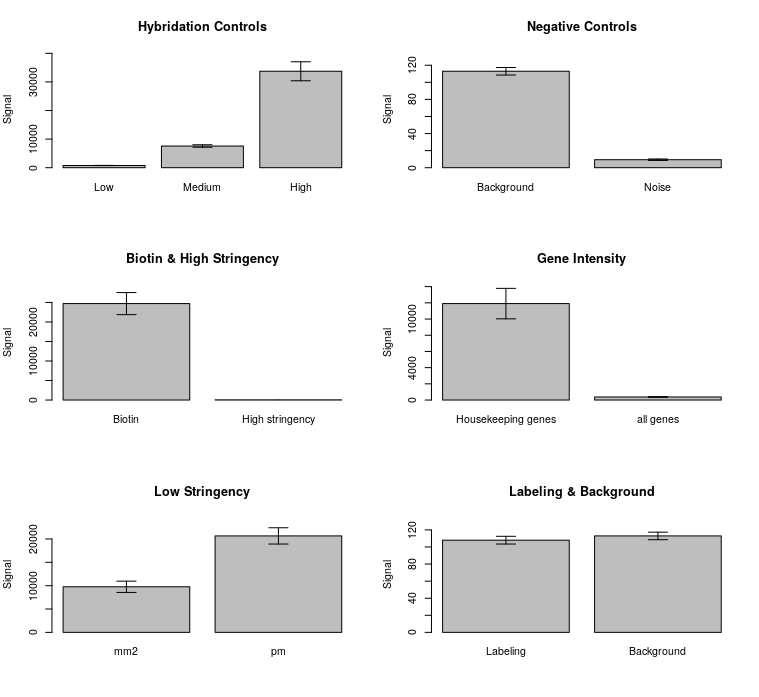
\includegraphics[scale=0.7]{../../R/output/SummaryControl.png}
 % SummaryControl.png: 0x0 pixel, 300dpi, 0.00x0.00 cm, bb=
 \captionof{figure}{Résume de l'ensemble de contôle d'hybridation direct de la technologie BeadArray d'Illumina}
\end{center}
\begin{center}
 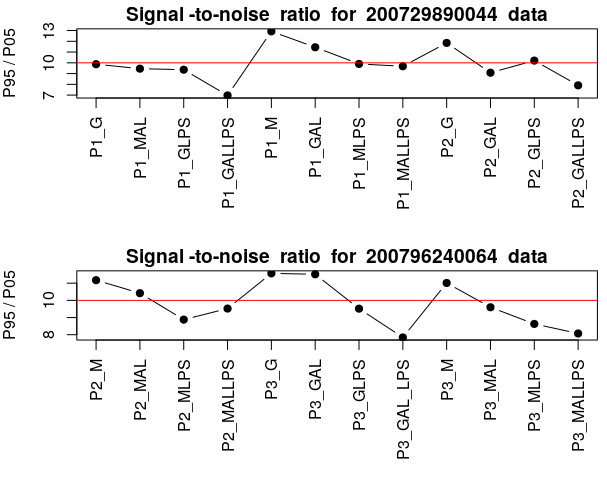
\includegraphics[scale=0.5]{../../R/output/signal_to_noise.png}
 % signal_to_noise.png: 0x0 pixel, 300dpi, 0.00x0.00 cm, bb=
 \captionof{figure}{Rapport signal-bruit sur les deux puces}
 Un rapport signal/bruit (SNR) peut être calculé en utilisant les mesures fournies par le scanner (dans le fichier metrics.txt) incluant les 95(P95) et 5(P05) quantiles de toutes les intensités de pixels de  l’image de chaque section. 
 Ces informations de mesures dépendent du paramètre de scanner et sont tout aussi utile pour l’évaluation de la qualité des données des échantillons ou bien pour évaluer si des échantillons semblent être des valeurs aberrantes. 
 Illumina recommande que le ratio SNR soit supérieur à 10 pour les puces HT-12.
\end{center}
\begin{center}
 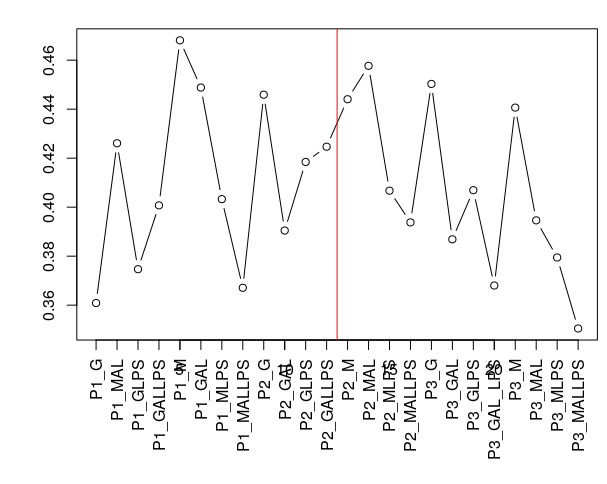
\includegraphics[scale=0.5]{../../R/output/propexpr.png}
 % propexpr.png: 0x0 pixel, 300dpi, 0.00x0.00 cm, bb=
 \captionof{figure}{ Estimation de proportion des sondes exprimées sur les deux puces avec la fonction propexpr() de limma}
 Ces valeurs ne sont pas vraiment des probabilités, elles estiment la proportion globale de sondes sur chaque section de la puce Illumina BeadChip qui correspondent à des gènes exprimés selon la méthode de Shi et al (2010).
 $pi1= (pb-p)/(pb-p1) $ avec $(pi1[pi1 > 1] \leftarrow 1 $ et $pi1[pi1 < 0] \leftarrow 0)$\\
 La fonction compare la distribution d’intensité empirique des sondes de contrôle négatif avec celle des sondes régulières. 
 Un modèle de mélange est adapté aux données de chaque échantillon de la puce pour inférer la distribution d’intensité des sondes exprimées et estimer la proportion exprimée.
\end{center}

\section{PR\'{E}TRAITEMENT DES DONN\'{E}ES :}
\subsection{Transformation :}
La distribution du niveau d'expression des gènes est très asymétrique avec un petit nombre de valeurs élevées. C’est une source de problèmes, car de nombreuses méthodes statistiques supposent implicitement une distribution gaussienne. 
Un simple calcul d’écart type ne satisfait donc pas de donner une interprétation habituelle de la distribution. La transformation logarithmique est la plus utilisée. 
\\Il y a plusieurs avantages d’utiliser la transformation logarithmique. Les données transformées sont plus faciles à interpréter (avec la variation du niveau d’expression des gènes plus réaliste) et aussi plus signifiantes de point de vue biologique (les intensités sont généralement comprises entre 0 et 65 535). 
L’asymétrie est fortement diminuée et la transformation  rend la distribution du niveau d’expression des gènes presque normale(distribution gaussienne).
Après transformation, les méthodes statistiques peuvent être utilisées en toute confiance. 
\subsection{Normalisation :}
Il n’est pas très judicieux de se lancer tout de suite à la comparaison et l’analyse des expressions des gènes à partir des échantillons multiples, car des sources parasites de variations des expressions peuvent fausser le résultat, exemples :quantité d’ARN différentes dans les échantillons, efficacité de la détection 
de fluorescence, biais systématiques, artefacts, conditions d’hybridation des échantillons.
Parmi ces sources, on cible plus précisément :
\begin{itemize}
 \item \emph{l’hétérogénéité du bruit de fond} :
 Si le bruit de fond présente des variations très différentes d’une puce à une autre, ou très structurées spatialement sur une puce, alors on peut être amené à corriger le signal par soustraction du bruit de fond. 
 \item \emph{l’hétérogénéité du signal} :
 De la même manière, le principe d’invariance d’une très grande majorité des expressions géniques d’une puce à une autre doit se traduire par une répartition comparable des valeurs des signaux entre les différentes puces. Si des différences marquées existent, il est judicieux de ramener les signaux moyens de chaque puce à la même valeur.
\end{itemize}
Avant de s’approcher des hypothèses favorables pour l’analyse différentielle, la normalisation est nécessaire afin de s’assurer que les données des différentes puces sont exploitables et comparable entre elles, que les différences d’intensité sont en effet dues à l’expression différentielle et non aux artefacts et les biais techniques expérimentaux.
Il y a plusieurs méthodes de normalisation souvent classé en deux catégories :
\begin{itemize}
 \item \emph{méthodes qui utilisent des données de référence (baseline array)}: scaling methods and non-linear methods
 \item \emph{méthodes qui combinent l’information de toutes les sections de la puce dans un ensemble de données donné (méthode complet)}: Lowess,normalisation par quantile,RMA(Robust Multi-Array Analysis)
\end{itemize}

% \subsection{Filtrage :}
\subsection{La fonction neqc() du package Limma :}
Le package Limma (écrit par Gordon Smyth,Matthew Ritchie et autres) contient pas mal de fonction de normalisation de puce à ADN que ce soit à une ou double couleur. Mais la fonction qui nous intéresse est la fonction neqc() spécialement personnalisée pour les puces Illumina BeadChips.
Cette fonction R effectue avant la transformation logarithmique des données une correction de bruit de fond utilisant des sondes de contrôle négatif suivie après par la normalisation par quantile utilisant à la fois les sondes de contrôle positif et négatif.
\\L’algorithme utilise le modèle « normexp » pour la correction de bruit de fond qui consiste à modéliser les intensités de pixels observées en tant que somme de deux variables aléatoires, une normalement distribuée et l’autre répartie exponentiellement, représentant respectivement le bruit et le signal de fond. 
La moyenne (\emph{mu}) et l’écart-type (\emph{sigma}) du bruit de fond normalement distribuée du modèle normexp sont estimés avec les valeurs des sondes de contrôle négatif et  la moyenne (\emph{alpha}) du signal répartie exponentiellement est estimée comme la différence entre la moyenne du signal et la moyenne des sondes de contrôle négatif.
\begin{scriptsize}
 \\$mu \leftarrow colMeans(xn, na.rm = TRUE)$
 \\$sigma \leftarrow sqrt(rowSums((t(xn) - mu)^2, na.rm = TRUE)/(nrow(xn) - 1))$
 \\$alpha \leftarrow pmax(colMeans(xr, na.rm = TRUE) - mu, 10)$
 \\$mu.sf \leftarrow x - mu - sigma^2/alpha$
 \\$signal \leftarrow mu.sf + sigma^2 * exp(dnorm(0, mean = mu.sf, sd = sigma, log = TRUE) - pnorm(0, mean = mu.sf, sd = sigma, lower.tail = FALSE, log.p = TRUE))$
\end{scriptsize}
\\Après la correction, un petit décalage (offset) est ajouté (par défaut 16) aux intensités corrigées pour  améliorer la performance dans la phase d’analyse d’expression différentielle et on applique la normalisation par quantile(\emph{normalizeBetweenArrays}).
Le but de la normalisation par quantile est de mettre la distribution, médiane et la moyenne des intensités des sondes de chaque puce sur le même niveau pour toutes les échantillons. Ceci est fait de façon suivante :
\begin{enumerate}
 \item Donner la matrice des intensités $X$ de dimensions $p * n$ avec les colonnes représentent les échantillons et les lignes représentent les sondes
\item Trier chaque colonne de X par ordre croissant pour construire $X_{sort}$
\item Calculer la moyenne par ligne de $X_{sort}$ et affecter cette moyenne sur chaque élément dans la ligne pour avoir $X_{sm}$
\item Construire $X_{normalized}$ en réarrangeant  les éléments de chaque colonne de Xsm dans l’ordre de la matrice  original $X$
\end{enumerate}
\begin{center}
 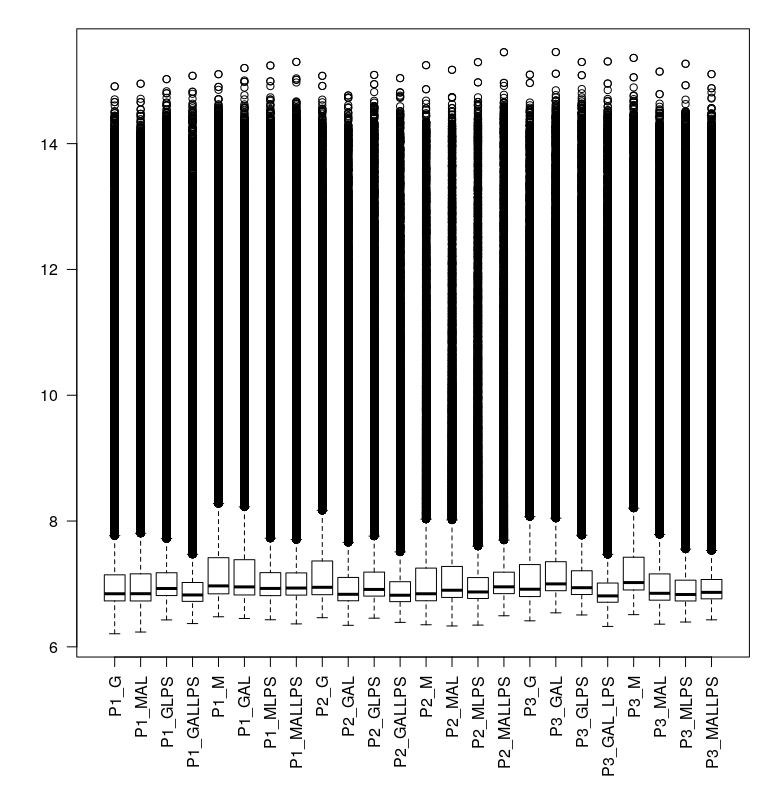
\includegraphics[scale=0.5]{../../R/output/boxplotbeforeNorm.png}
 % boxplotbeforeNorm.png: 0x0 pixel, 300dpi, 0.00x0.00 cm, bb=
 \captionof{figure}{ Box plot des signaux avant normalisation}
\end{center}
\begin{center}
 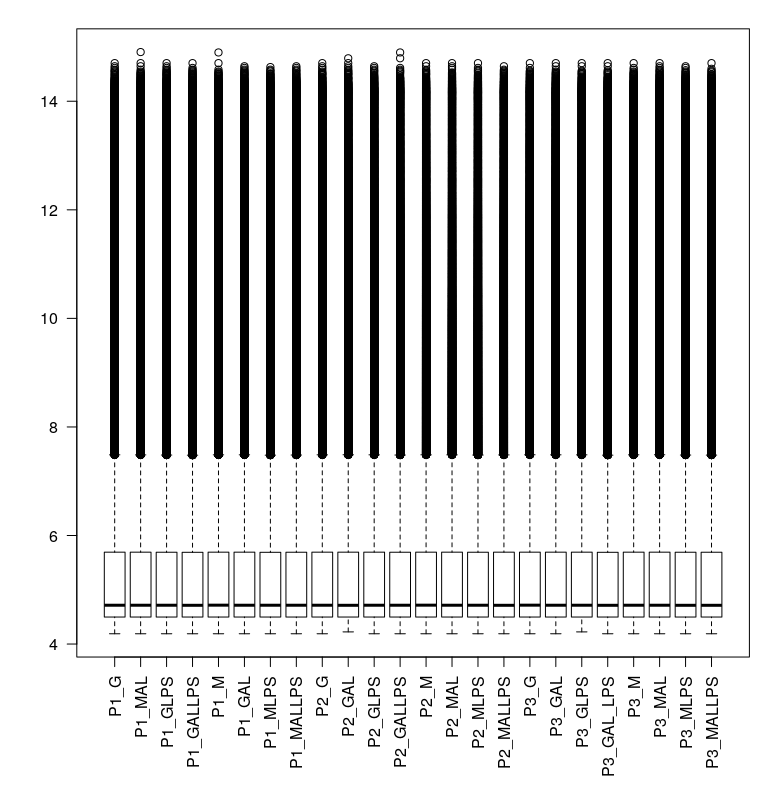
\includegraphics[scale=0.5]{../../R/output/boxplotAfterNorm.png}
 % boxplotbeforeNorm.png: 0x0 pixel, 300dpi, 0.00x0.00 cm, bb=
 \captionof{figure}{ Box plot des signaux après normalisation}
\end{center}
\begin{center}
 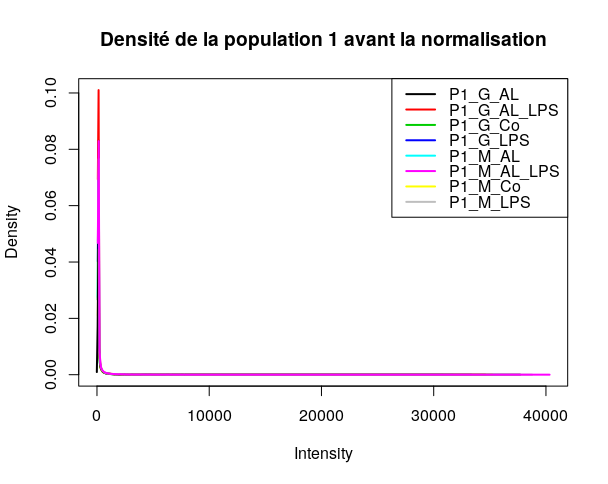
\includegraphics[scale=0.5]{../../R/output/Densitypop1.png}
 % Densité_pop1.png: 0x0 pixel, 300dpi, 0.00x0.00 cm, bb=
 \captionof{figure}{ Densité de la population 1 avant la normalisation}
\end{center}
\begin{center}
 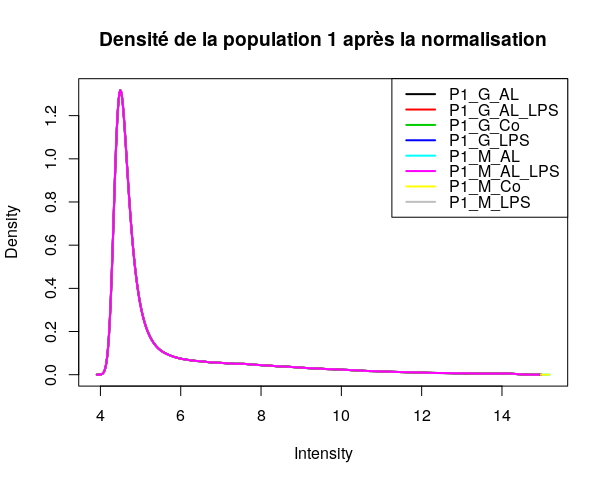
\includegraphics[scale=0.5]{../../R/output/Densitypop1C.png}
 % Densité_pop1(correct).png: 0x0 pixel, 300dpi, 0.00x0.00 cm, bb=
 \captionof{figure}{ Densité de la population 1 après la normalisation}
\end{center}

\section{ANALYSE DES DONN\'{E}ES DE TRANSCRIPTOME :}
% \subsection{Gènes différentiellement exprimés :}
% \subsection{Gènes co-exprimés :}
=> En cours
\section{INTERP\'{E}TATION :}
=> Pas de temps
% (Caractérisation d’un ensemble de gènes)
\section{CONCLUSION :}
\end{document}          
